\capitulo{3}{Metodología}

\section{Descripción de los datos.}
%Breve descripción de los datos.
%En caso de tratarse de un trabajo donde los datos son muy importantes, puede haber explicaciones extra en el anexo correspondiente.

Este apartado resume el análisis de las señales obtenidas por medio del uso de dos sensores inerciales, un acelerómetro y un giroscopio, cuyos parámetros están correlacionados con los síntomas motores parkinsonianos y, de esta forma, ofrecer información relevante a la hora de detectar la discinesia y la bradicinesia entre otros. 

Una vez se han adquirido las señales, se deberán filtrar para eliminar el ruido y, así evitar que interfiera en la calidad. Se procederá a la selección y extracción de características que representen las distintas actividades motoras mediante el uso de filtros paso banda y ventanas deslizantes, cuyos parámetros se definirán en base a estudios realizados y los empleados en el diseño del dispositivo KinetiSense \cite{mera2013quantitative}, el sistema PERFORM \cite{tzallas2014perform} tanto para el acelerómetro como para el giroscopio. 

Asimismo, los resultados obtenidos son introducidos como parámetros de entrada en diferentes algoritmos de clasificación (Regresión logística, SVM, Random forest, AdaBoost), los cuales serán comparados para establecer el algoritmo que garantice la correcta clasificación de cada uno de los síntomas motores.


En el \textit{Anexo Descripción de adquisición y tratamiento de datos} se explica de forma detallada las características de las señales que devuelven los acelerómetros y los giroscopios, así como la presencia de tablas que muestren los parámetros de los filtros pasa banda y de las ventanas deslizantes empleados para caracterizar los síntomas parkinsonianos. 
 
\section{Técnicas y herramientas.}

%Esta parte de la memoria tiene como objetivo presentar las técnicas metodológicas y las herramientas de desarrollo que se han utilizado para llevar a cabo el proyecto. Si se han estudiado diferentes alternativas de metodologías, herramientas, bibliotecas se puede hacer un resumen de los aspectos más destacados de cada alternativa, incluyendo comparativas entre las distintas opciones y una justificación de las elecciones realizadas. 
%No se pretende que este apartado se convierta en un capítulo de un libro dedicado a cada una de las alternativas, sino comentar los aspectos más destacados de cada opción, con un repaso somero a los fundamentos esenciales y referencias bibliográficas para que el lector pueda ampliar su conocimiento sobre el tema.


\subsection{Herramientas}

Teniendo en cuenta las especificaciones técnicas de los dispositivos actuales del mercado, para el desarrollo del dispositivo se va a requerir de:
\begin{itemize}
    \item Microcontrolador
    \item Cable USB
    \item Acelerómetro/Giroscopio
    \item Módulo Bluetooth
    \item Módulo WiFi
\end{itemize}

Actualmente existe gran variedad de microcontroladores y, en concreto, en este proyecto se va a trabajar con Arduino, una plataforma de código abierto que se utiliza para programar dispositivos electrónicos debido a su facilidad de uso. Consta de dos partes \cite{badamasi2014working}:  
\begin{enumerate}
    \item Hardware: se trata de una placa de circuito con chip programable que permite realizar diferentes tareas y está constituido por diversos componentes combinados para su funcionamiento, incluyendo el microcontrolador y pines de alimentación de 3,3 V a 5 V (Figura \ref{fig:placa-arduino}). Es capaz de leer información proveniente de dispositivos de entrada como sensores, así como enviar información a dispositivos de salida e incluso a través de Internet para controlar el dispositvo electrónico.
    
    A diferencia de otras placas de circuito programables, a través de un cable USB se puede cargar código nuevo en la placa sin necesidad de una pieza de hardware separada.
    
    \item Software (Arduino IDE): emplea una versión simplificada de C++ e incluye el conjunto de instrucciones que el hardware va a realizar.
\end{enumerate}

 \begin{figure}[ht]
    \centering
    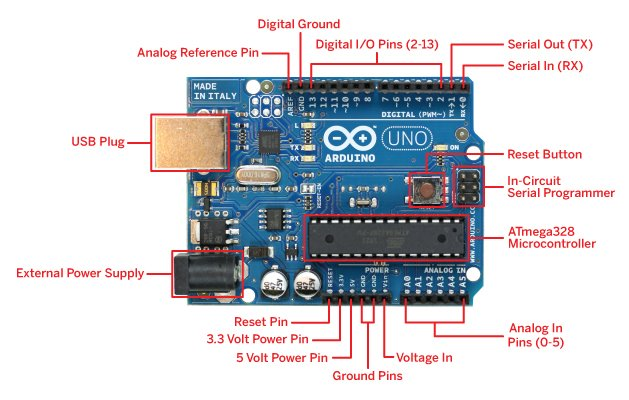
\includegraphics[width=0.7\textwidth]{img/arduino.jpg}
    \caption{Componentes de la placa de Arduino uno \cite{website:aprendiendoarduino.wordpress} }
    \label{fig:placa-arduino}
 \end{figure}


Observando que los distintos dispositivos orientados al análisis del estado motor de los pacientes de Parkinson presentan un acelerómetro y un giroscopio para evaluar la bradicinesia y la discinesia, se va a emplear el sensor MPU6050 (Figura \ref{fig:MPU6050}). 

El sensor MPU6050 es una unidad de medición inercial (IMU) de 6 grados de libertad que combina un giroscopio de 3 ejes para medir la velocidad angular y un acelerómetro de 3 ejes. 

Además, la comunicación puede realizarse tanto por SPI como por bus I2C. La tensión de alimentación es de 2.4 V a 3.6 V y una de las ventajas es su bajo precio \cite{website:luisllamas-mpu, website:naylampmechatronics}. 

\begin{figure}[ht]
        \centering
        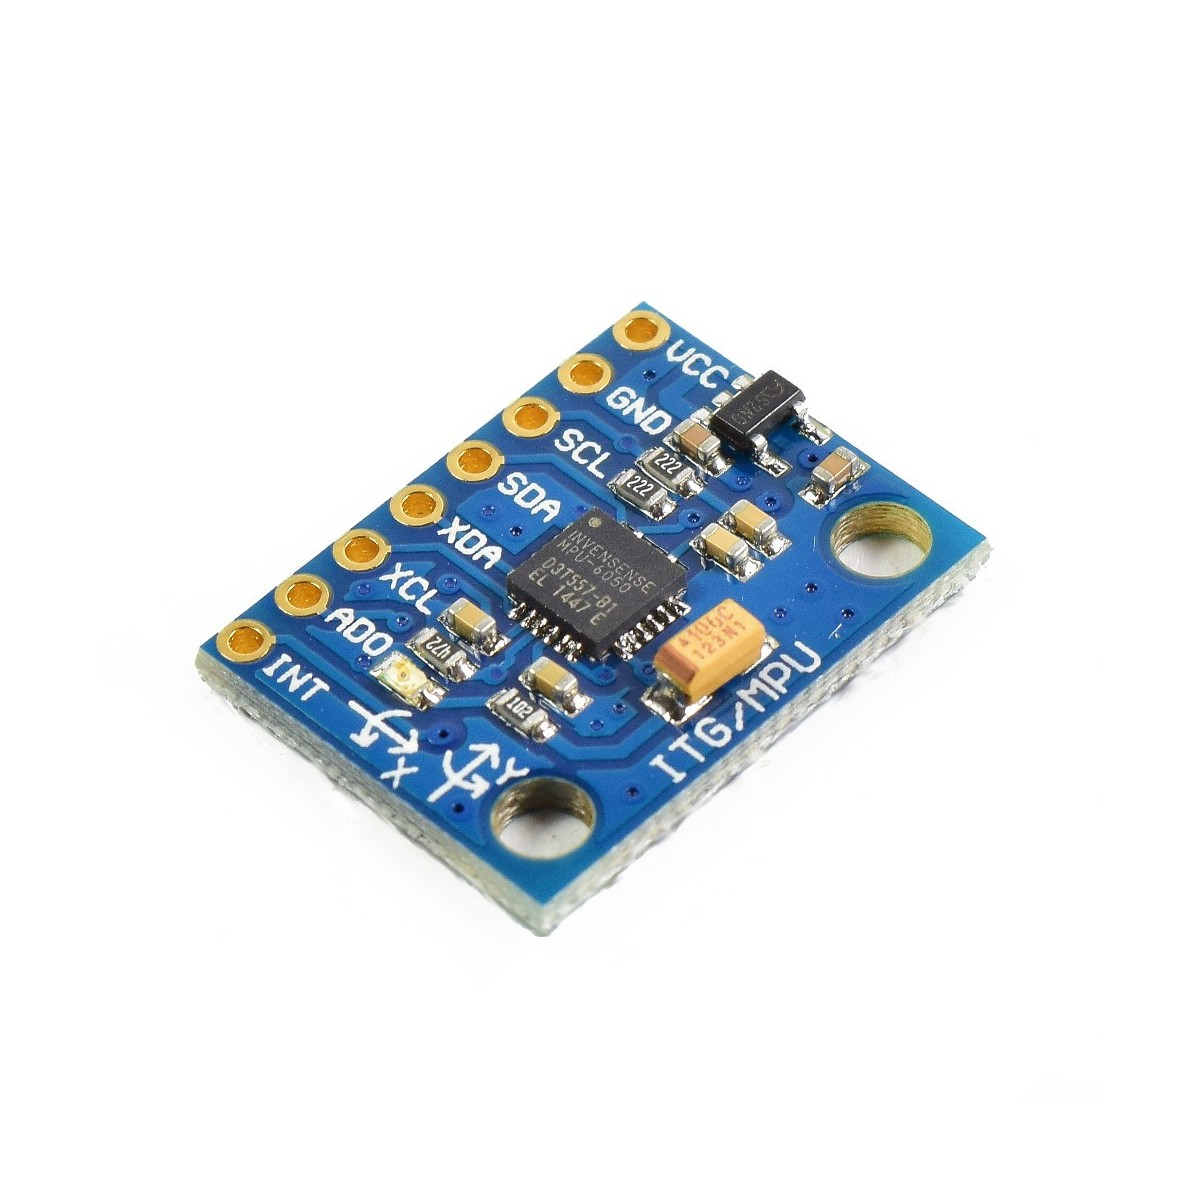
\includegraphics[width=0.35\textwidth]{img/modulo6050.jpg}
        \caption{Sensor MPU6050: acelerómetro y giroscopio  \cite{website:naylampmechatronics} }
        \label{fig:MPU6050}
\end{figure}

Para realizar la lectura del sensor MPU6050, se emplearán dos biblioteca de Arduino desarrolladas por Jeff Rowberg \cite{website:github.com/jrowberg}, una para MPU6050 y una segunda para la comunicación I2C.

Por otra parte, se ha valorado el empleo de módulos Bluetooth y WiFi para que los resultados sean enviados al servidor web para su posterior análisis.

\begin{itemize}
    \item Módulo HC-05: como se muestra en la Figura \ref{fig:HC-O5}, módulo Bluetooth es de pequeño tamaño, el cual permite conectar de forma sencilla un Arduino por Bluetooth y es capaz de recibir e iniciar comunicaciones, a diferencia del módulo Hc-06.
    
    A través del propio Serial Monitor del Arduino IDE se puede realizar la conexión entre el módulo y nuestro dispositivo. Uno de sus inconvenientes es que requiere el uso de puerto serie de la placa Arduino \cite{website:luisllamas-BT}.

    \begin{figure}[ht]
        \centering
        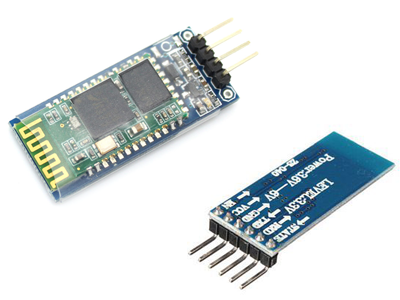
\includegraphics[width=0.35\textwidth]{img/arduino-bluetooth-hc05.png}
        \caption{Módulo Bluetooth HC-O5  \cite{website:luisllamas-BT} }
        \label{fig:HC-O5}
    \end{figure}

    \item Módulo ESP8266 WiFi de tipo ESP01: se trata de un módulo de bajo coste con Wifi integrado cuyo diseño se muestra en la Figura \ref{fig:ESP8266}. La conexión con Arduino es sencilla, pero la principal dificultad es la alimentación, ya que tiene una tensión de alimentación de 3,3 V y, en caso de alimentarse a una tensión superior a 3,6 V, el módulo se dañará \cite{website:luisllamas-wifi}. 

    \begin{figure}[ht]
        \centering
        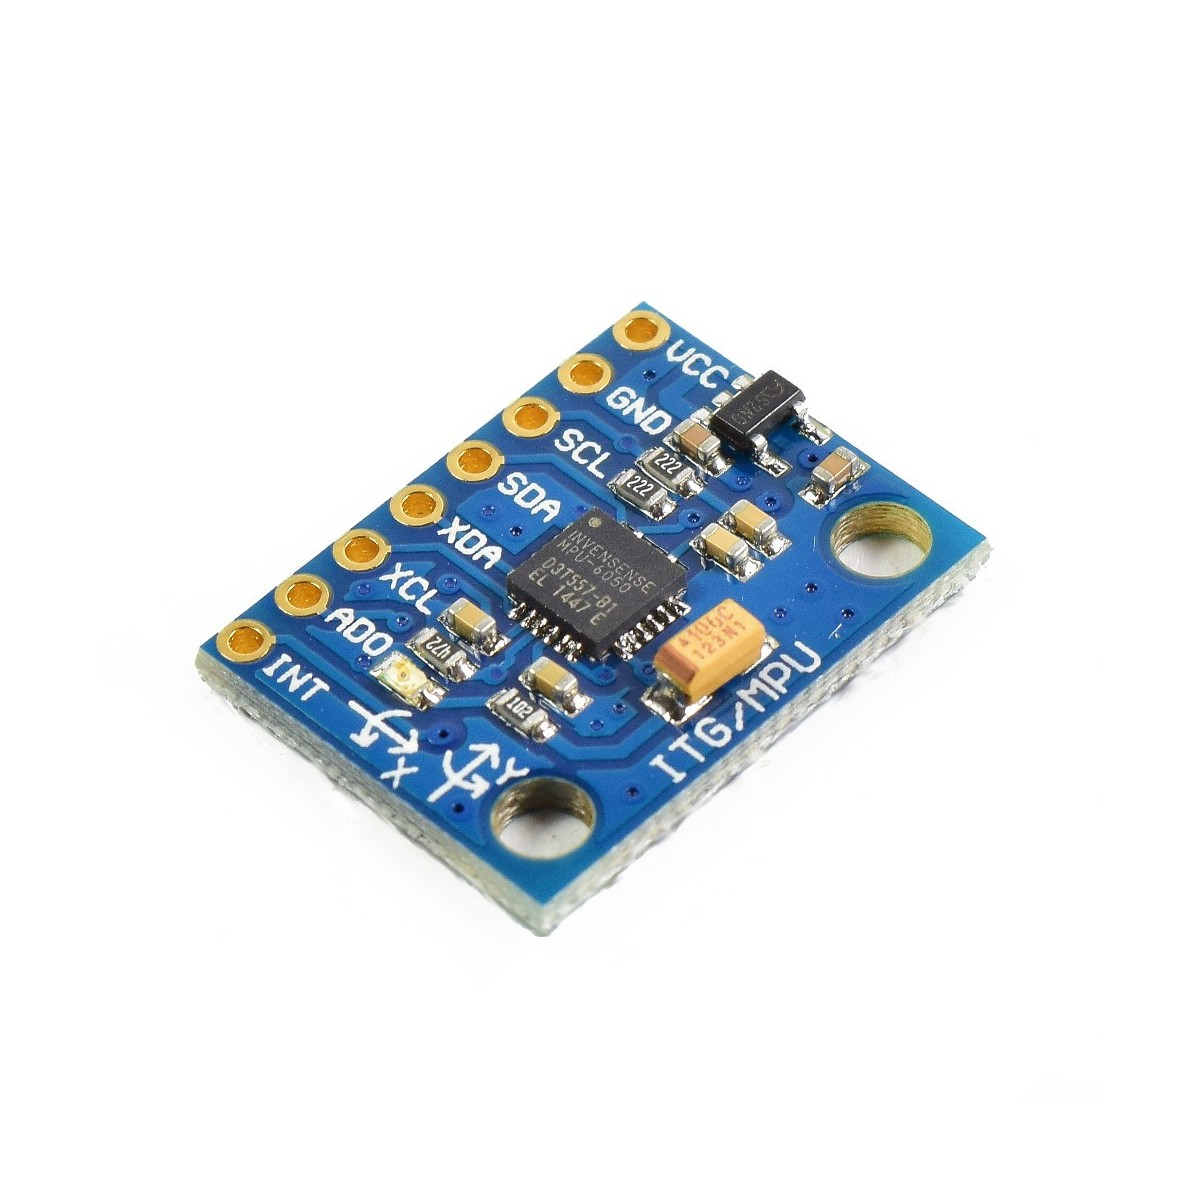
\includegraphics[width=0.35\textwidth]{img/modulo6050.jpg}
        \caption{Módulo ESP8266 WiFi de tipo ESP01  \cite{website:descubrearduino} }
        \label{fig:ESP8266}
    \end{figure}
\end{itemize}

\subsection{Algoritmos de aprendizaje supervisado - Clasificación}

Una vez adquiridos los datos, se emplearán distintos algoritmos de aprendizaje supervisado para clasificarlos en función de los síntomas característicos de la enfermedad de Parkinson.
Los algoritmos que mayormente se han empleando para la clasificación de actividades motoras son los siguientes:

\begin{enumerate}
    \item Regresión logística: algoritmo utilizado ampliamente por su simplicidad para predecir la probabilidad de que un evento que tiene un resultado dictómico (binario) esté relacionado con un conjunto de variables \cite{muniz2010comparison}. 
    \item SVM (Support Vector Machine): algoritmo que define un límite de decisión (hiperplano) que divide de forma óptima dos clases al maximizar la distancia entre ellas.  Busca los vectores de soporte  que ofrezcan el mejor hiperplano de separación empleando una función kernel \cite{bourouhou2016comparison}.
    \item Random Forest: algoritmo supervisado capaz de realizar tareas de regresión y clasificación. Consiste en ejecutar varios algoritmos de árbol de decisiones, en el que cada uno da una clasificación. La decisión final será aquella que aparezca más veces \cite{liaw2002classification}.
	\item AdaBoost:
\end{enumerate}


